\nuovapagina

\vs(15)
{\normalsize \bf Fase 1)}\\
\vs(10)
{\normalsize \bf Attenuazione degli elementi di disturbo: peli}
\vs(5)

\fbox{
\noindent
\begin{minipage}{16cm}
\vs(10)
\bfl
\centerline{
  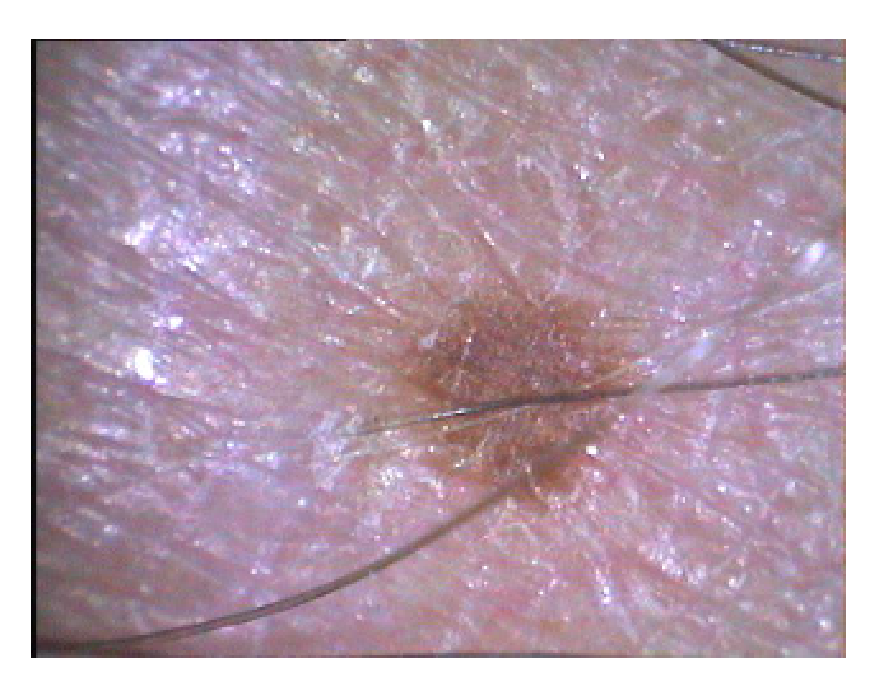
\psfig{file="./images/cpeli.eps",height=6cm,clip=}
  \hfill
  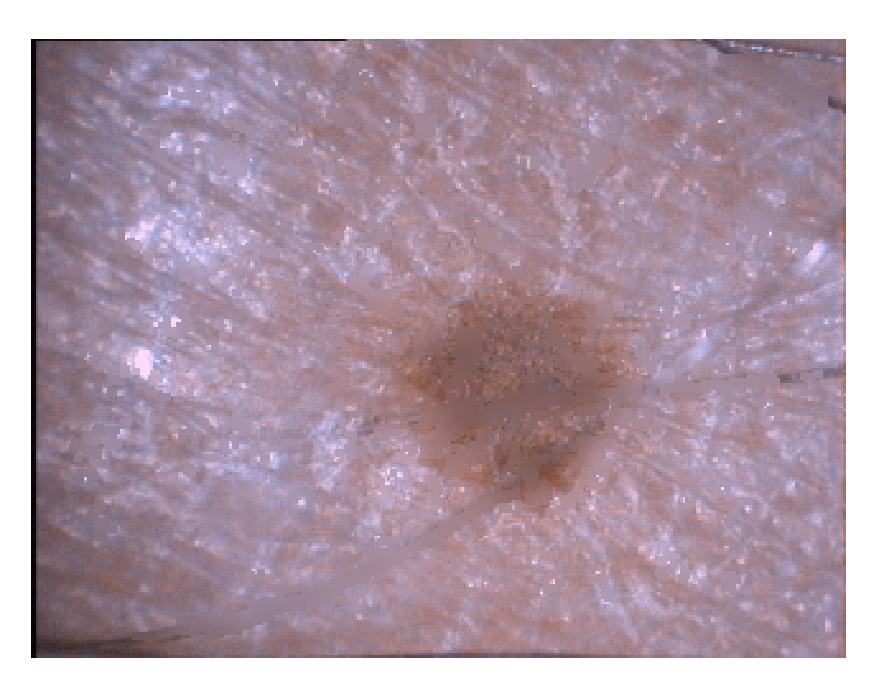
\psfig{file="./images/spelio.eps",height=6cm,clip=}
}
\os(20) Originale \os(35)  Operatore Anisotropo\\
\vs(20)
\centerline{
 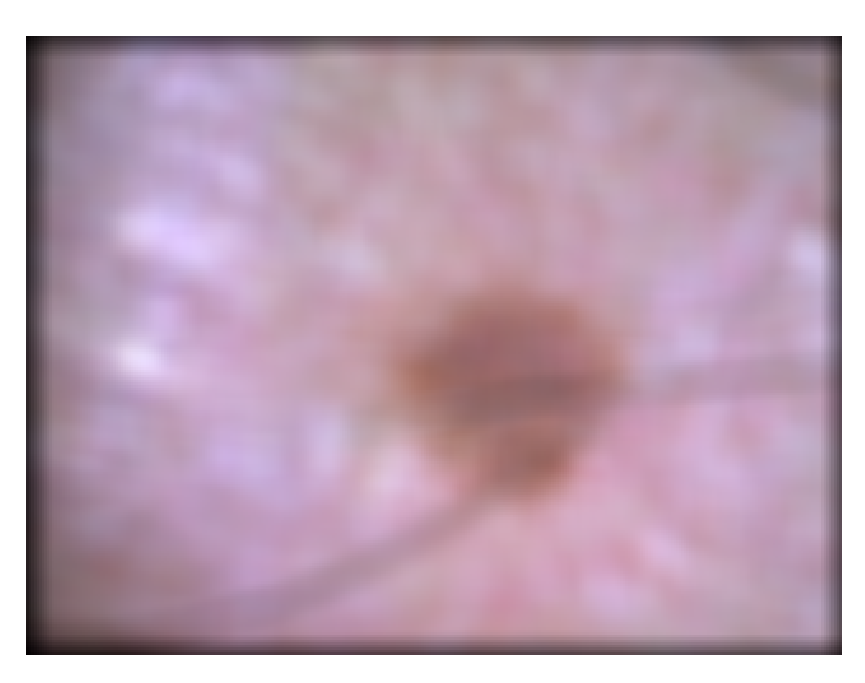
\psfig{file="./images/spelig.eps",height=5cm,clip=}
 \hfill
 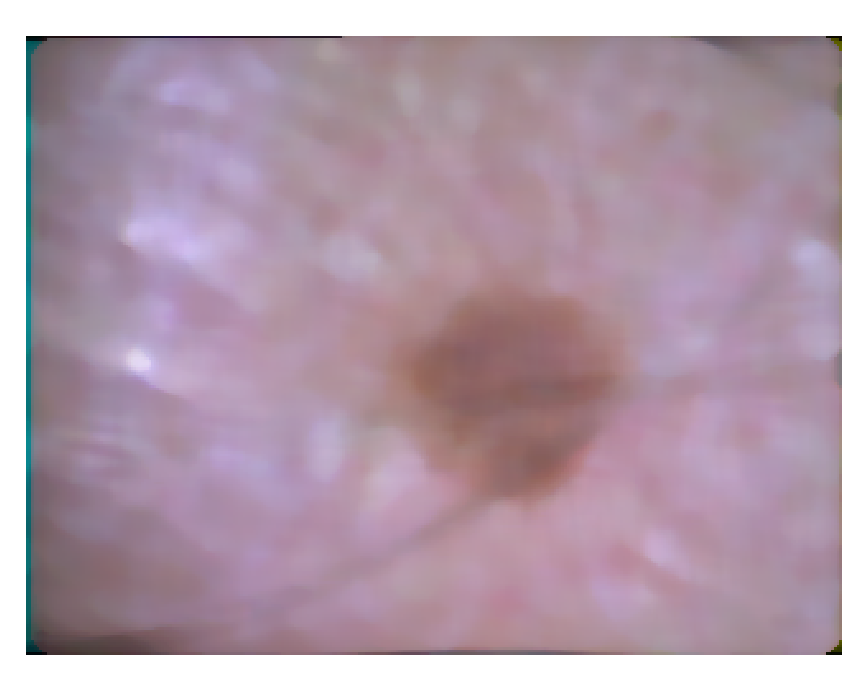
\psfig{file="./images/spelim.eps",height=5cm,clip=}
}
\os(3) Filtro PB Gaussiano \os(32) Filtro a mediana\\
\vs(10)
\efl
\end{minipage}
}

%===========================================================================================
\nuovapagina

\vs(3)
{\normalsize \bf Inizializzazione automatica dello snake}

\fbox{
\noindent
\begin{minipage}{16cm}
\vs(2)
\bfl
\bi
\im Trasformata di Karhunen-Lo\`eve (o di Hotelling) dell'immagine a colori originale
\im Binarizzazione della componente principale

    \centerline{
     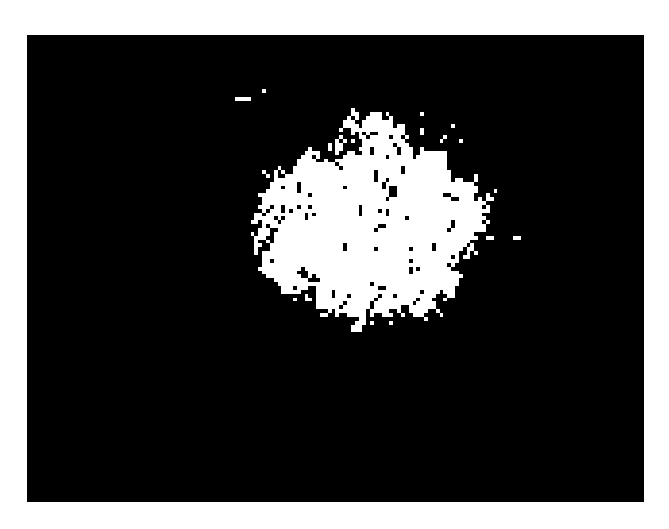
\psfig{file="./images/neobin2.eps",height=6cm,clip=} 
    }
\im Elaborazione con operatori morfologici:
    \bi
    \im {\it apertura}: per eliminare piccoli disturbi isolati e l'eccessiva frastagliatura
    \im {\it chiusura}: con un nucleo circolare per ottenere una unica regione compatta
                        e con bordi regolari

    \centerline{
     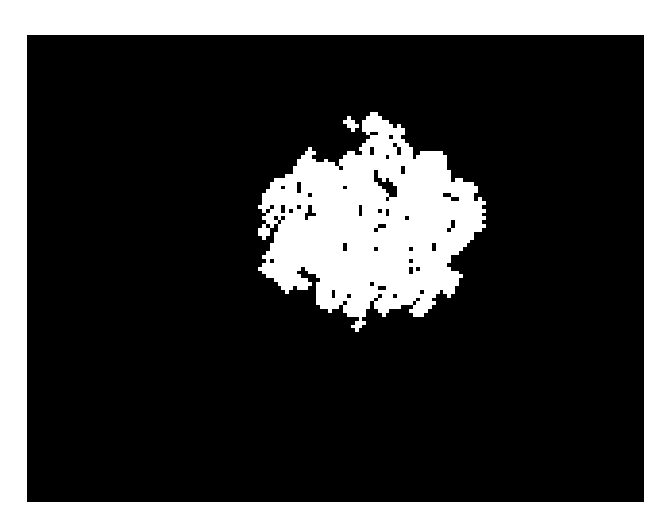
\psfig{file="./images/neobo2.eps",height=6cm,clip=}
     \hfill 
     
\psfig{file="./images/neoboc2.eps",height=6cm,clip=}
    }
    \ei
\im La curva iniziale \e ottenuta a partire dal bordo della regione appena ricavata
\ei 
\efl
\vs(5)
\end{minipage}
}

